\section{Vizuelizacija i grafički dizajn}
Iako je tekst glavni sadržaj jednog časopisa, on mora biti i vizuelno privlačan čitaocima. Zbog toga časopis ima i grafički odsek u kome su zaposleni ljudi vični krojenju izgleda kako štampanih tako i digitalnih strana. \\

Pored fotografa i ilustratora koji stvaraju potpuno nove slike iz ničega, u grafičkom odseku rade i dizajneri; profesionalci koji uklapanjem celina, izborom boja i tipografije prave prikaz na čije elemente većina čitaoca ne obraća pažnju ali koji igra ogromnu ulogu u ostavljenom utisku. \\

Celim odeskom rukovodi grafički urednik koji je osoba istančanog osećaja za izgled i dizajn. Njegova uloga je prvenstveno kritička, sav vizuelni materijal koji se u izdavaštvu proizvede on mora odobriti, on mora znati kako da d\^{a} pravi savet koji će pomoći stvaraocu da dovede svoj rad na nivo prihvatljiv standardima časopisa.


\begin{figure}[htb]
    \centering
    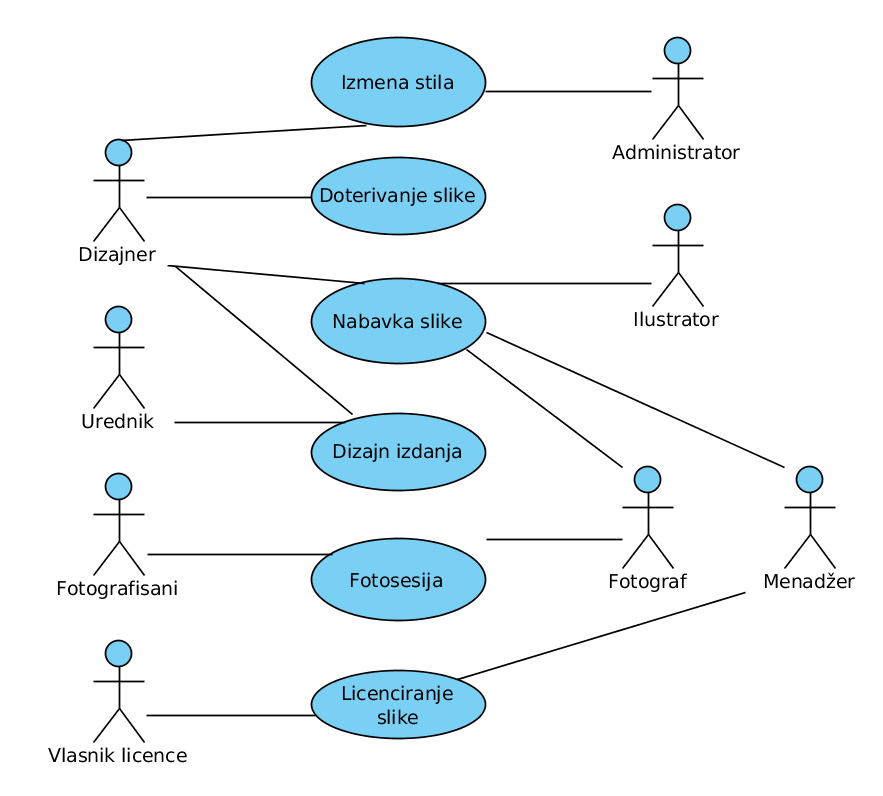
\includegraphics[width=0.7\textwidth]{slike/upotreba_grafika}
    \caption{Dijagram slučajeva upotrebe - pisanje članka}
    \label{grafika}
\end{figure}

\subsection{Dizajniranje štampanog članka}
\begin{description}
\item [Opis] Grafički urednik sa svojim saradnicima kreira i određuje kako će članak u štampanom izdanju izgledati.
\item [Učesnici] (Grafički) urednik, dizajner, ilustrator (fotograf).
\item [Ulaz] Članak u tekstualnom obliku.
\item [Izlaz] Članak ukrašen i ukomponovan sa ostatkom izdanja.
\item [Preduslov] Članak je napisan i neće trpeti veće promene nadalje.
\item [Postuslov] Izgled članka je određen.
\end{description}
\subsubsection{Glavni tok}
\begin{enumerate} 
\item Urednik prima tekst članka.
\item Urednik zadužuje dizajnera za rad na članku, dajući mu predloge ukoliko ih ima.
\item Dizajner bira sliku kojom će ilustrovati članak. Pred njim su tri izbora:
\begin{enumerate}
\item Može upotrebiti sliku koja već postoji u bazi podataka.
\item Može zadužiti ilustratora (ili fotografa) da proizvede željenu sliku.
\item Može naći sliku drugde i zatražiti pravnom odseku (menadžmentu) da je licencira.
\end{enumerate}
\item Dizajner prilagođava sliku potrebama članka,
uklapa je prostorno i stvara celokupan izgled stranica na kojima će se nalaziti članak.
\item Dizajner predaje svoj rad uredniku koji ili:
\begin{enumerate}
\item Odobrava predatu verziju kao završnu i dodaje je u konačnu verziju izdanja.
\item Ili nudi kritiku dizajneru i vraća ga na korak 3 ili korak 4 ukoliko je zamerka manja.
\end{enumerate}
\end{enumerate}
\subsubsection{Alternativni tok}
Ukoliko usred prevelikog obima posla ili tehničkih nemogućnosti ilustratori (fotografi) zaposleni u izdavaštvu ne mogu napraviti željenu sliku, unajmljuje se hororarni ilustrator (fotograf).

\subsection{Dizajniranje internet članka}
\begin{description}
\item [Opis] Grafički urednik sa svojim saradnicima kreira i određuje kako će članak u štampanom izdanju izgledati.
\item [Učesnici] (Grafički) urednik, dizajner, ilustrator (fotograf).
\item [Ulaz] Članak u tekstualnom obliku.
\item [Izlaz] Ilustrovani članak u internet izdanju.
\item [Preduslov] Članak je napisan i neće trpeti veće promene nadalje.
\item [Postuslov] Izgled članka je određen.
\end{description}
\subsubsection{Glavni tok}
\begin{enumerate} 
\item Urednik prima tekst članka.
\item Urednik zadužuje dizajnera za rad na članku, dajući mu predloge ukoliko ih ima.
\item Dizajner bira sliku kojom će ilustrovati članak. Pred njim su tri izbora:
\begin{enumerate}
\item Može upotrebiti sliku koja već postoji u bazi podataka.
\item Može zadužiti ilustratora (ili fotografa) da proizvede željenu sliku.
\item Može naći sliku drugde i zatražiti pravnom odseku (menadžmentu) da je licencira.
\end{enumerate}
\item Dizajner prilagođava sliku potrebama članka, bira gde će se u tekstu nalaziti.
\item Dizajner predaje svoj rad uredniku koji ili:
\begin{enumerate}
\item Odobrava predatu verziju kao završnu i prosleđuje je administratoru koji objavljuje članak na veb stranici.
\item Ili nudi kritiku dizajneru i vraća ga na korak 3.
\end{enumerate}
\end{enumerate}
\subsubsection{Alternativni tok}
Ukoliko usred prevelikog obima posla ili tehničkih nemogućnosti ilustratori (fotografi) zaposleni u izdavaštvu ne mogu napraviti željenu sliku, unajmljuje se hororarni ilustrator (fotograf).

\subsection{Promena stila veb sajta}
\begin{description}
\item [Opis] Grafički urednik sa svojim saradnicima menja izgled sajta časopisa.
\item [Učesnici] (Grafički) urednik, dizajner, administrator.
\item [Ulaz] Trenutni izgled sajta (.css dokument).
\item [Izlaz] Novi izgled sajta (.css dokument).
\item [Preduslov] Sajt radi normalno.
\item [Postuslov] Sajt radi isto, ima novi izgled.
\end{description}
\subsubsection{Glavni tok}
\begin{enumerate} 
\item Urednik osmišlja novi izgled sajta.
\item Urednik predočava svoju zamisao dizajneru.
\item Dizajner određuje elemente stila, geometriju, boje, tipografiju. Pravi manje slike koje se koriste kao ikonice.
\item Dizajner predaje svoj rad uredniku koji ili:
\begin{enumerate}
\item Odobrava i predaje rezultat administratoru koji ga podešava kao novi izgled stranice.
\item Ili nudi kritiku dizajneru i vraća ga na korak 3.
\end{enumerate}
\end{enumerate}
\subsubsection{Alternativni tok}
Ukoliko promene dovedu do nepredviđenih problema kasnije, stari stil se može privremeno vratiti dok se rešenje ne nađe.

\subsection{Dizajn naslovne strane}
\begin{description}
\item [Opis] Uredništvo zajedno sa dizajnerima osmišlja i kreira naslovnu stranu štampanog izdanja.
\item [Učesnici] Glavni urednik, Grafički urednik, ostali urednici, dizajneri.
\item [Ulaz] Nema.
\item [Izlaz] Naslovna strana.
\item [Preduslov] Sadržaj novog izdanja je okvirno poznat.
\item [Postuslov] Naslovna strana za iduće izdanje je napravljena.
\end{description}
\subsubsection{Glavni tok}
\begin{enumerate} 
\item Uredništvo (Glavni i grafički sa izvršnim urednicima) se okuplja i razmenjuje ideje za naslovnu stranu,
 uključujući pored slike koja će biti prikazana i koji članci će biti promovisani na njoj.
\item Glavni urednik bira najbolju od predloženih ideja.
\item Grafički urednik nadograđuje ideju detaljima za koje misli da bi načinili bolju sliku i zadužuje grafičke radnike da rade na njoj.
\item Nabavlja se osnovna slika tako što:
\begin{enumerate}
\item Ilustrator stvara sliku bilo ručno ili pomoću programa ili u nekoj kombinaciji.
\item Fotograf slika osobu, predmet ili prizor koji je zatražen.
\item Licencira se već postojeća slika.
\end{enumerate}
\item Dizajner dodaje promotivne naslove članaka, usklađuje boje i slično i predaje svoj rad grafičkom uredniku koji:
\begin{enumerate}
\item Odobrava i predaje rezultat glavnom uredniku.
\item Ili nudi kritiku dizajneru i vraća ga na korak 3.
\end{enumerate}
\item Glavni urednik isto tako kritikuje ili odobrava, ukoliko je odobreno to se smatra konačnom verzijom i biva štampano sa ostatkom izdanja. 
\end{enumerate}
\subsubsection{Alternativni tok}
U nedostatku prihvatljivih ideja od strane uredništva, grafičkom odseku se može dati veća kreativna sloboda pri kreiranju stranice. Ova svejedno mora proći kroz odobrenje grafičkog i glavnog urednika.

\begin{figure}[htbp]
    \centering
    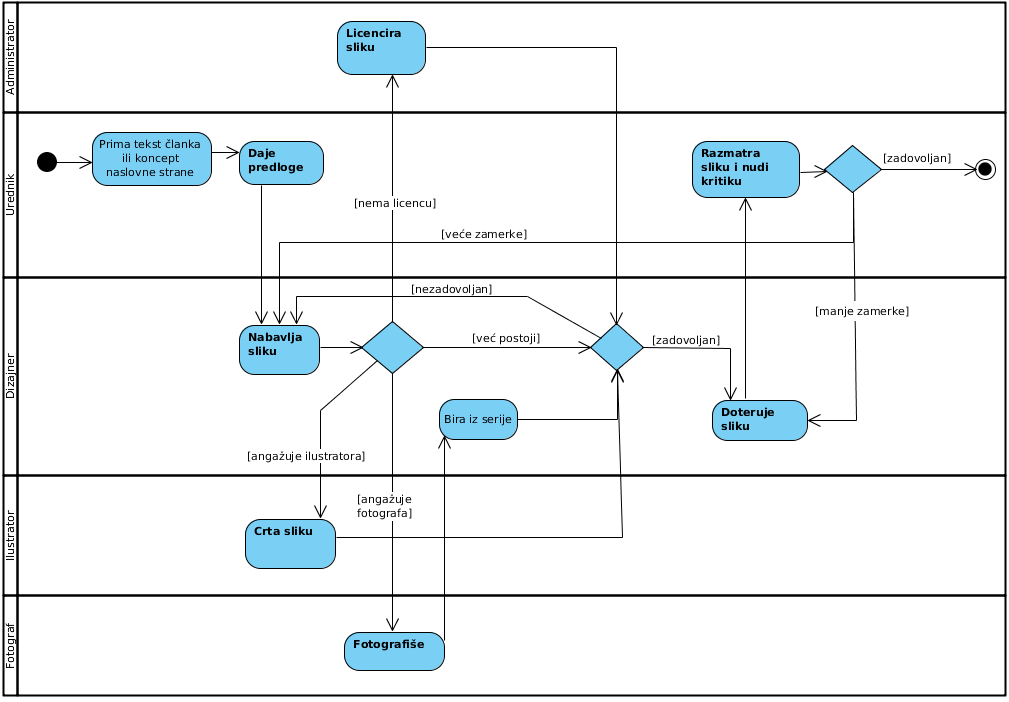
\includegraphics[height=0.4\textheight]{slike/grafika}
    \caption{Dijagram aktivnosti - Dizajn članka ili naslovne strane}
    \label{grafika}
\end{figure}

\subsection{Pravljenje fotoportreta}
\begin{description}
\item [Opis] Fotograf pravi fotografiju osobe.
\item [Učesnici] Fotograf, fotografisani (često intervjuisani), grafički urednik.
\item [Ulaz] Nema.
\item [Izlaz] Profesionalna fotografija osobe.
\item [Preduslov] Osoba je pristala da se slika za časopis.
\item [Postuslov] Slika je spremna da se upotrebi u časopisu.
\end{description}
\subsubsection{Glavni tok}
\begin{enumerate} 
\item Fotograf i osoba se nalaze na dogovorenom mestu: studiju ili na mestu gde je osoba intervjuisana.
\item Fotograf namešta potrebnu opremu i pravi niz fotografija sa osobom.
\item Fotograf sa grafičkim urednikom bira najpogodniju fotografiju iz niza.
\end{enumerate}
\subsubsection{Alternativni tokovi}
\begin{enumerate} 
\item Ukoliko osoba povuče svoj pristanak u bilo kom momentu posao se obustavlja.
\item Ukoliko nijedna fotografija nije prihvatljiva slikanje se može ponoviti, mada se ovo izbegava jer bi bilo neprijatno za osobu koja se slika.
\end{enumerate}

\subsection{Licenciranje slike}
\begin{description}
\item [Opis] Administracija se na zahtev grafičkog dizajnera dogovara sa vlasnikom licence da otkupi prava na upotrebu slike.
\item [Učesnici] Dizajner, Menadžer, vlasnik.
\item [Ulaz] Nema.
\item [Izlaz] Zvanična dozvola za upotrebu slike.
\item [Preduslov] Dizajner zna koja mu je slika potrebna i vlasnik prava se može naći.
\item [Postuslov] Časopis može legalno koristiti sliku.
\end{description}
\subsubsection{Glavni tok}
\begin{enumerate} 
\item Grafički dizajner nalazi sliku koja mu je potrebna, obično preko Interneta ili drugih izdanja.
\item Menadžer pronalazi ko je vlasnik licence za sliku i kako ga kontaktirati.
\item Menadžer otkupljuje potrebna prava.
\end{enumerate}
\subsubsection{Alternativni tok}
Ukoliko vlasnik ne želi dati pravo ili ga je ne moguće kontaktirati ili je cena licence previsoka odustaje se od licenciranja.